\subsection{Geographic Analysis -- Where are the data?}

% [Word comment] (on "36,000") This can't be right, but this was using Yubin's
% old table that had public data marked and using only public data. However in
% the new table we don't have lat/lon corrdinates for this many gauges show
The dataset consists of over 37,000 gauges. The dataset contains data from 126 countries based on the World Bank country boundaries. We analyzed the geographic location of the gauges and present an analysis to summarize where the data are primarily available and where they are missing. The figure below shows the location of almost 36,000 of the gauges. The map marks which stations for discharge versus stage data.

\begin{figure}[!htbp]
\centering
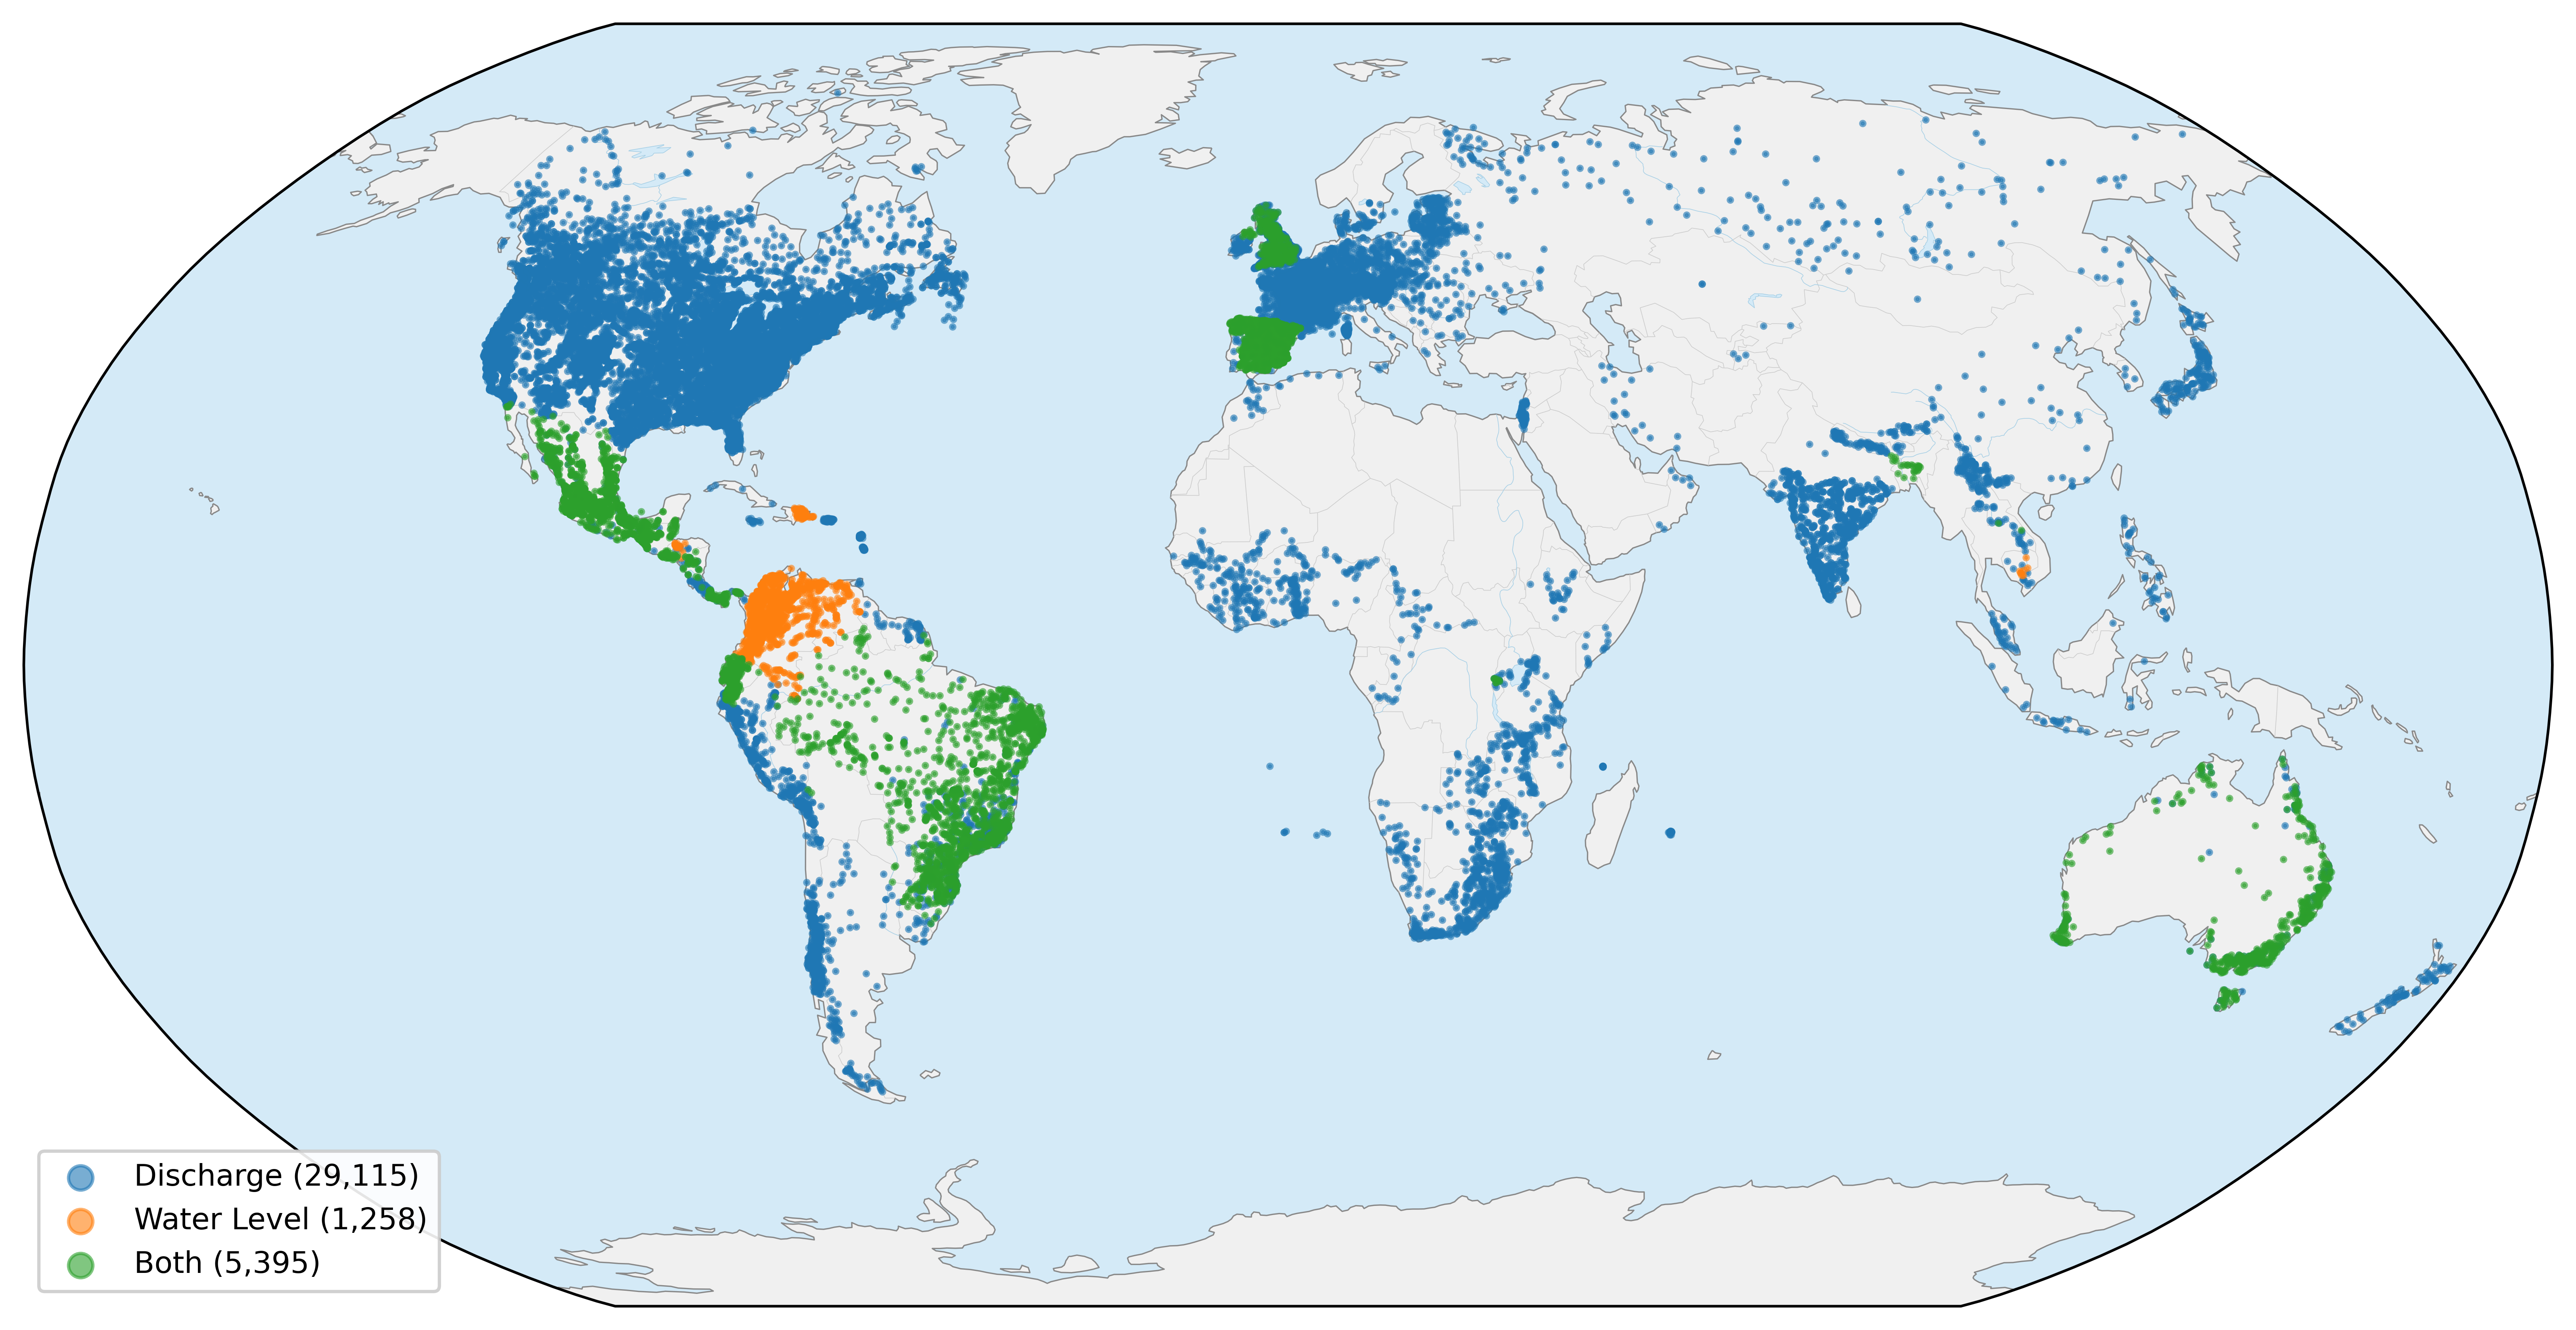
\includegraphics[width=\textwidth]{figures/fig01_gauge_locations.png}
\caption{Locations of publicly available gauges, marked by whether they report discharge, water level, or both.}
\label{fig:gauge-locations}
\end{figure}

Examining the figure shows some interesting patterns in spatial biases around the world. This dataset does not have much data in the Nile River Basin. While we know data exists in that area, data sharing protocols prevent it from being included in global datasets. We also note that as expected there are very few gauges in areas that are primarily desert including in the Sahara Desert, the Arabian desert, Patagonia, and the Australian desert. We also note from this figure that certain areas of the world, such as Europe, the United States and Canada, are much more densely covered than other areas. The United States contains over 11,000 gauges making up about a third of the dataset.

In the dataset, there are 113 countries and territories without any gauge data. However, many of the countries are smaller islands such as Maldives, a land locked but small country such as Vatican City, or a small territory owned by another country such as Guam. The following figure shows the area size of countries. Many of the countries are smaller than the United States state of Rhode Island which is a little smaller than 3000 square kilometers. Therefore, while the number of countries missing gauges is high, the amount of area is much smaller.

The following figure shows the sizes of countries with no gauges compared with the sizes of countries with gauges. It is graphed on a log scale to show all the countries. The figure shows that most of the small countries do not have gauges, but large countries tend to have gauges. This demonstrates that even while the number of countries and territories without gauges is high, the amount of area is much smaller. The figure also shows that there are some large countries that do not have gauges, such as Greenland, Western Sahara, and Libya.

\begin{figure}[!htbp]
\centering
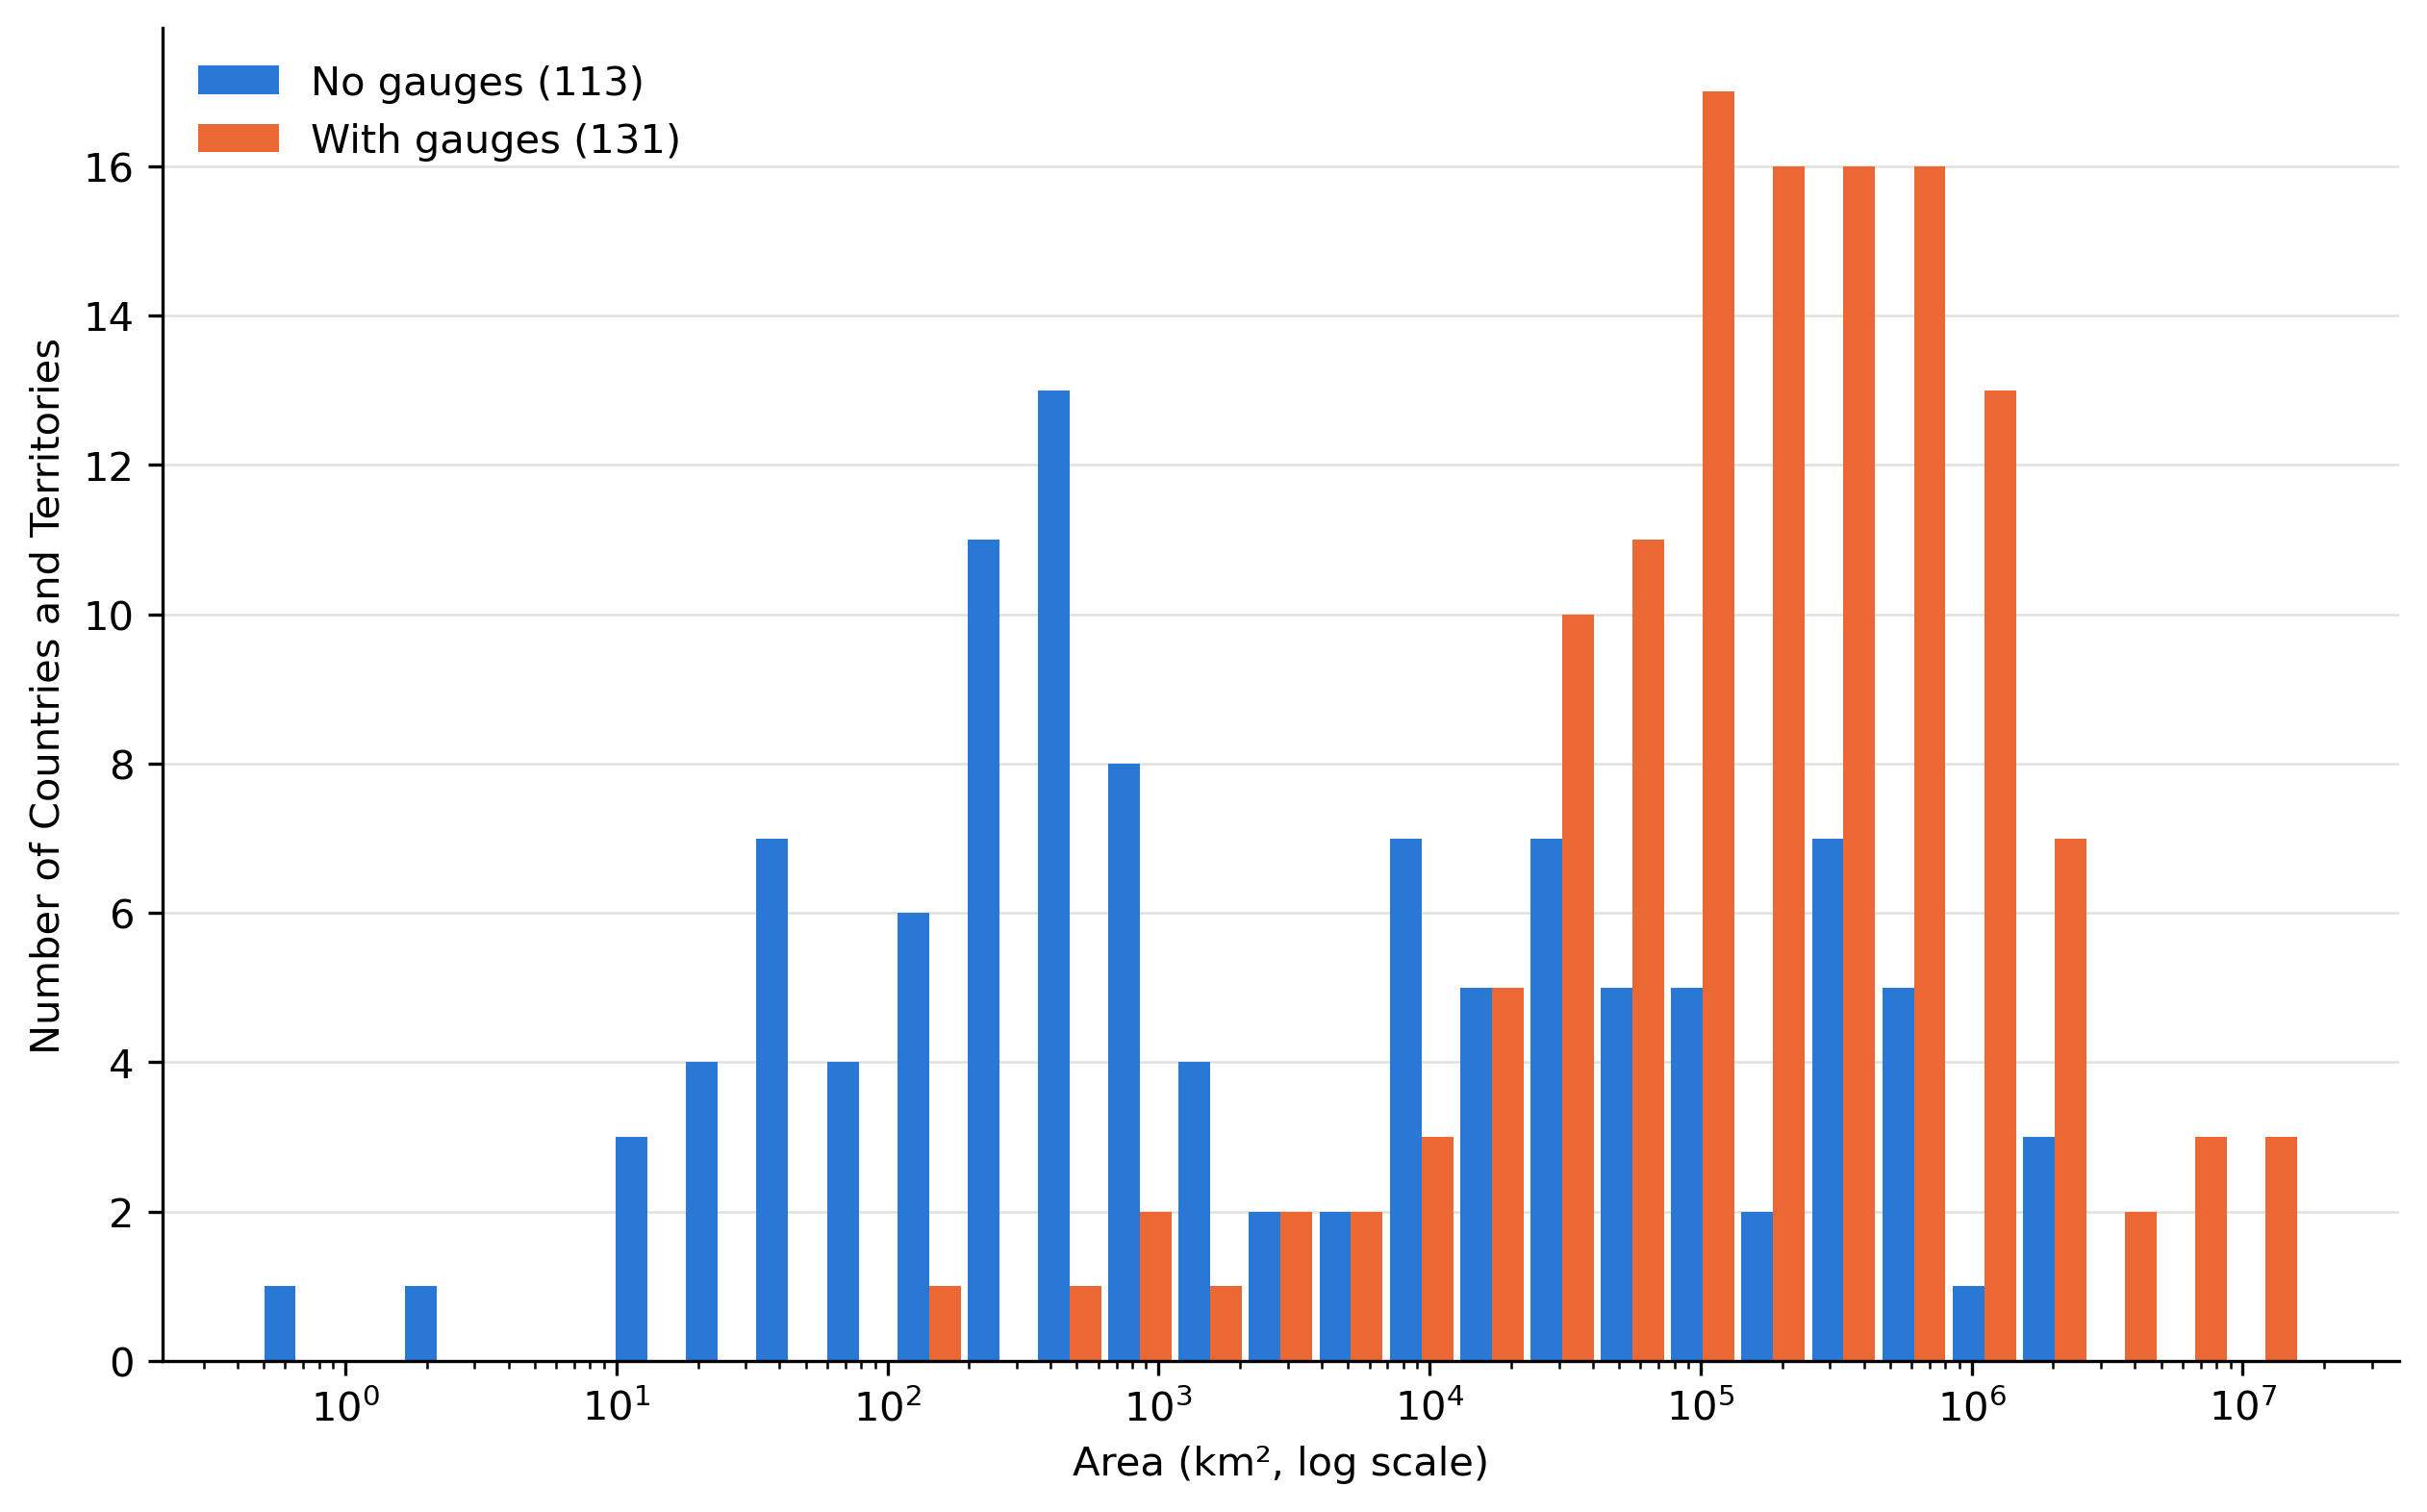
\includegraphics[width=\textwidth]{figures/fig02_country_areas.png}
\caption{Distribution of the areas of countries with no gauges.}
\label{fig:country-areas}
\end{figure}

We examined to see if the countries with data were biased at all based on income levels. The World Bank calssifies countries on income levels based on Gross National Income (GNI) per capita. The World Bank classifies countries as low income, lower middle income, upper middle income and high income. This analysis is redone every year. For this paper, we used the given classifications for fiscal year 2025 which were made effective July 1, 2026.The following table shows the thresholds for each of these categories.


\begin{table}[!htbp]
\centering
\caption{World Bank income classification thresholds for FY2027 (GNI per capita in 2025, current US\$, Atlas method).}
\label{tab:gni-categories}
\begin{tabular}{@{}ll@{}}
\toprule
Low Income & GNI $\leq$ \$1,175 \\
Lower Middle Income & \$1,176 -- \$4,635 \\
Upper Middle Income & \$4,636 -- \$14,375 \\
High Income & GNI $>$ \$14,375 \\
\bottomrule
\end{tabular}
\end{table}

We also examined each income group for how many people and area there were on average per gauge. In this analysis, the United States gauges were removed. This is because there are many gauges in the United States in our dataset that it had a significant impact on the averages of high-income category. Therefore, it was removed to give a more representative result.

% [Word comment] Should this table be redone to include countries that had no
% gauges?
\begin{table}[!htbp]
\centering
\caption{Average gauge counts, population, and area per gauge by income group, excluding the United States.}
\label{tab:income-groups}
\small
% Generated by figures_src/tab_income_groups.py
% Generated by figures_src/tab_income_groups.py -- do not edit by hand.
\begin{tabular}{@{}lC{0.14\textwidth}C{0.14\textwidth}C{0.14\textwidth}C{0.14\textwidth}@{}}
\toprule
Income Group & Average gauges per country & People per gauge (thousands) & Land area per gauge (1000 km\textsuperscript{2}) & Countries with gauges \\
\midrule
Low Income & 9.32 & 3,293.95 & 63.05 & 16 \\
Lower Middle Income & 44.19 & 1,418.05 & 9.09 & 33 \\
Upper Middle Income & 125.14 & 417.03 & 6.02 & 33 \\
High Income & 190.77 & 66.05 & 2.66 & 43 \\
\bottomrule
\end{tabular}

\end{table}

The following map shows the countries that are missing data grouped by incomes based on the GNI. There are countries with higher income that have no gauges in the dataset, but many of these countries have explanations for why no data may exist. Iceland is a smaller island and therefore does not have any major rivers. Finland and Norway similarly do not have many large rivers due to the coastlines, and both are north with lots of snow. The map shows that many of the countries missing data are in Northern Africa and Western Asia.

\begin{figure}[!htbp]
\centering
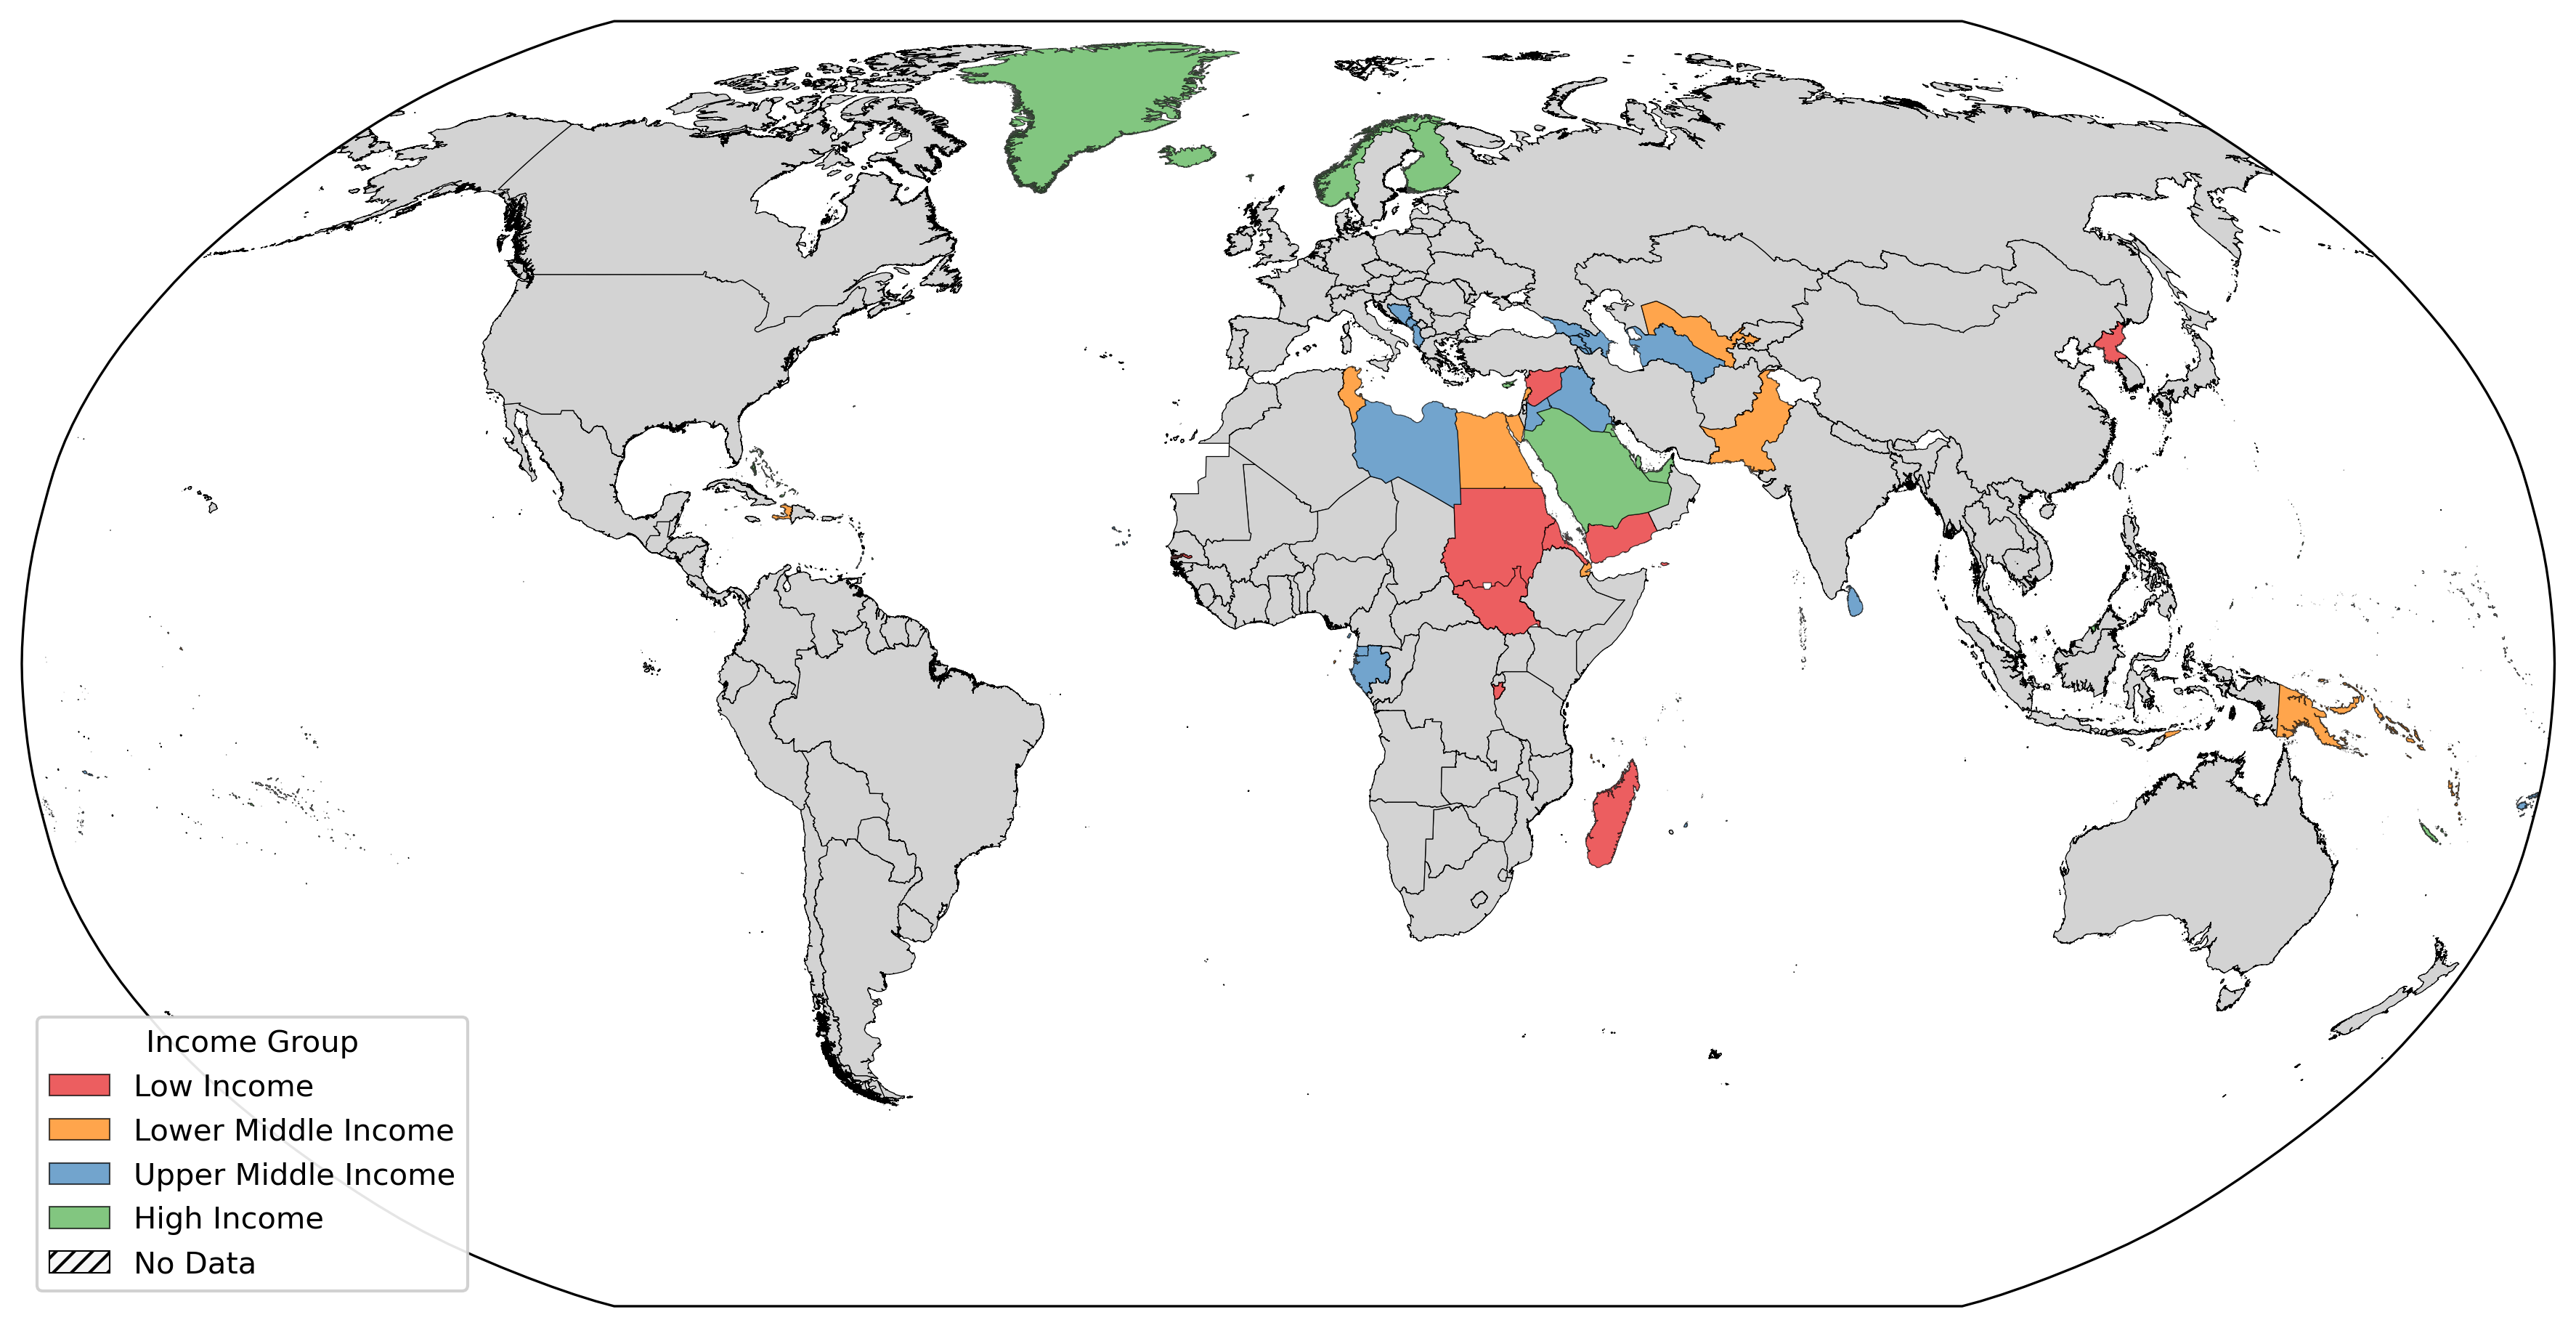
\includegraphics[width=\textwidth]{figures/fig03_missing_countries_income.png}
\caption{Countries with no gauges, grouped by income category based on GNI.}
\label{fig:missing-countries-income}
\end{figure}

% [Word comment] (on the Koppen sentence) Did this use the same one referenced
% in the methods section?
In addition to looking at which countries have data, we also observed which climate zones have more data available. We looked at the representation of gauges in the different Koppen Climate zones.

The largest portion of the gauges are in the temperate climate despite being the smallest percentage of land area. However, this is the climate with the greatest population of people. There are very few gauges in the polar regions, which could be due both to the lack of people living there as well as the lack of rivers to analyze.

\begin{figure}[!htbp]
\centering
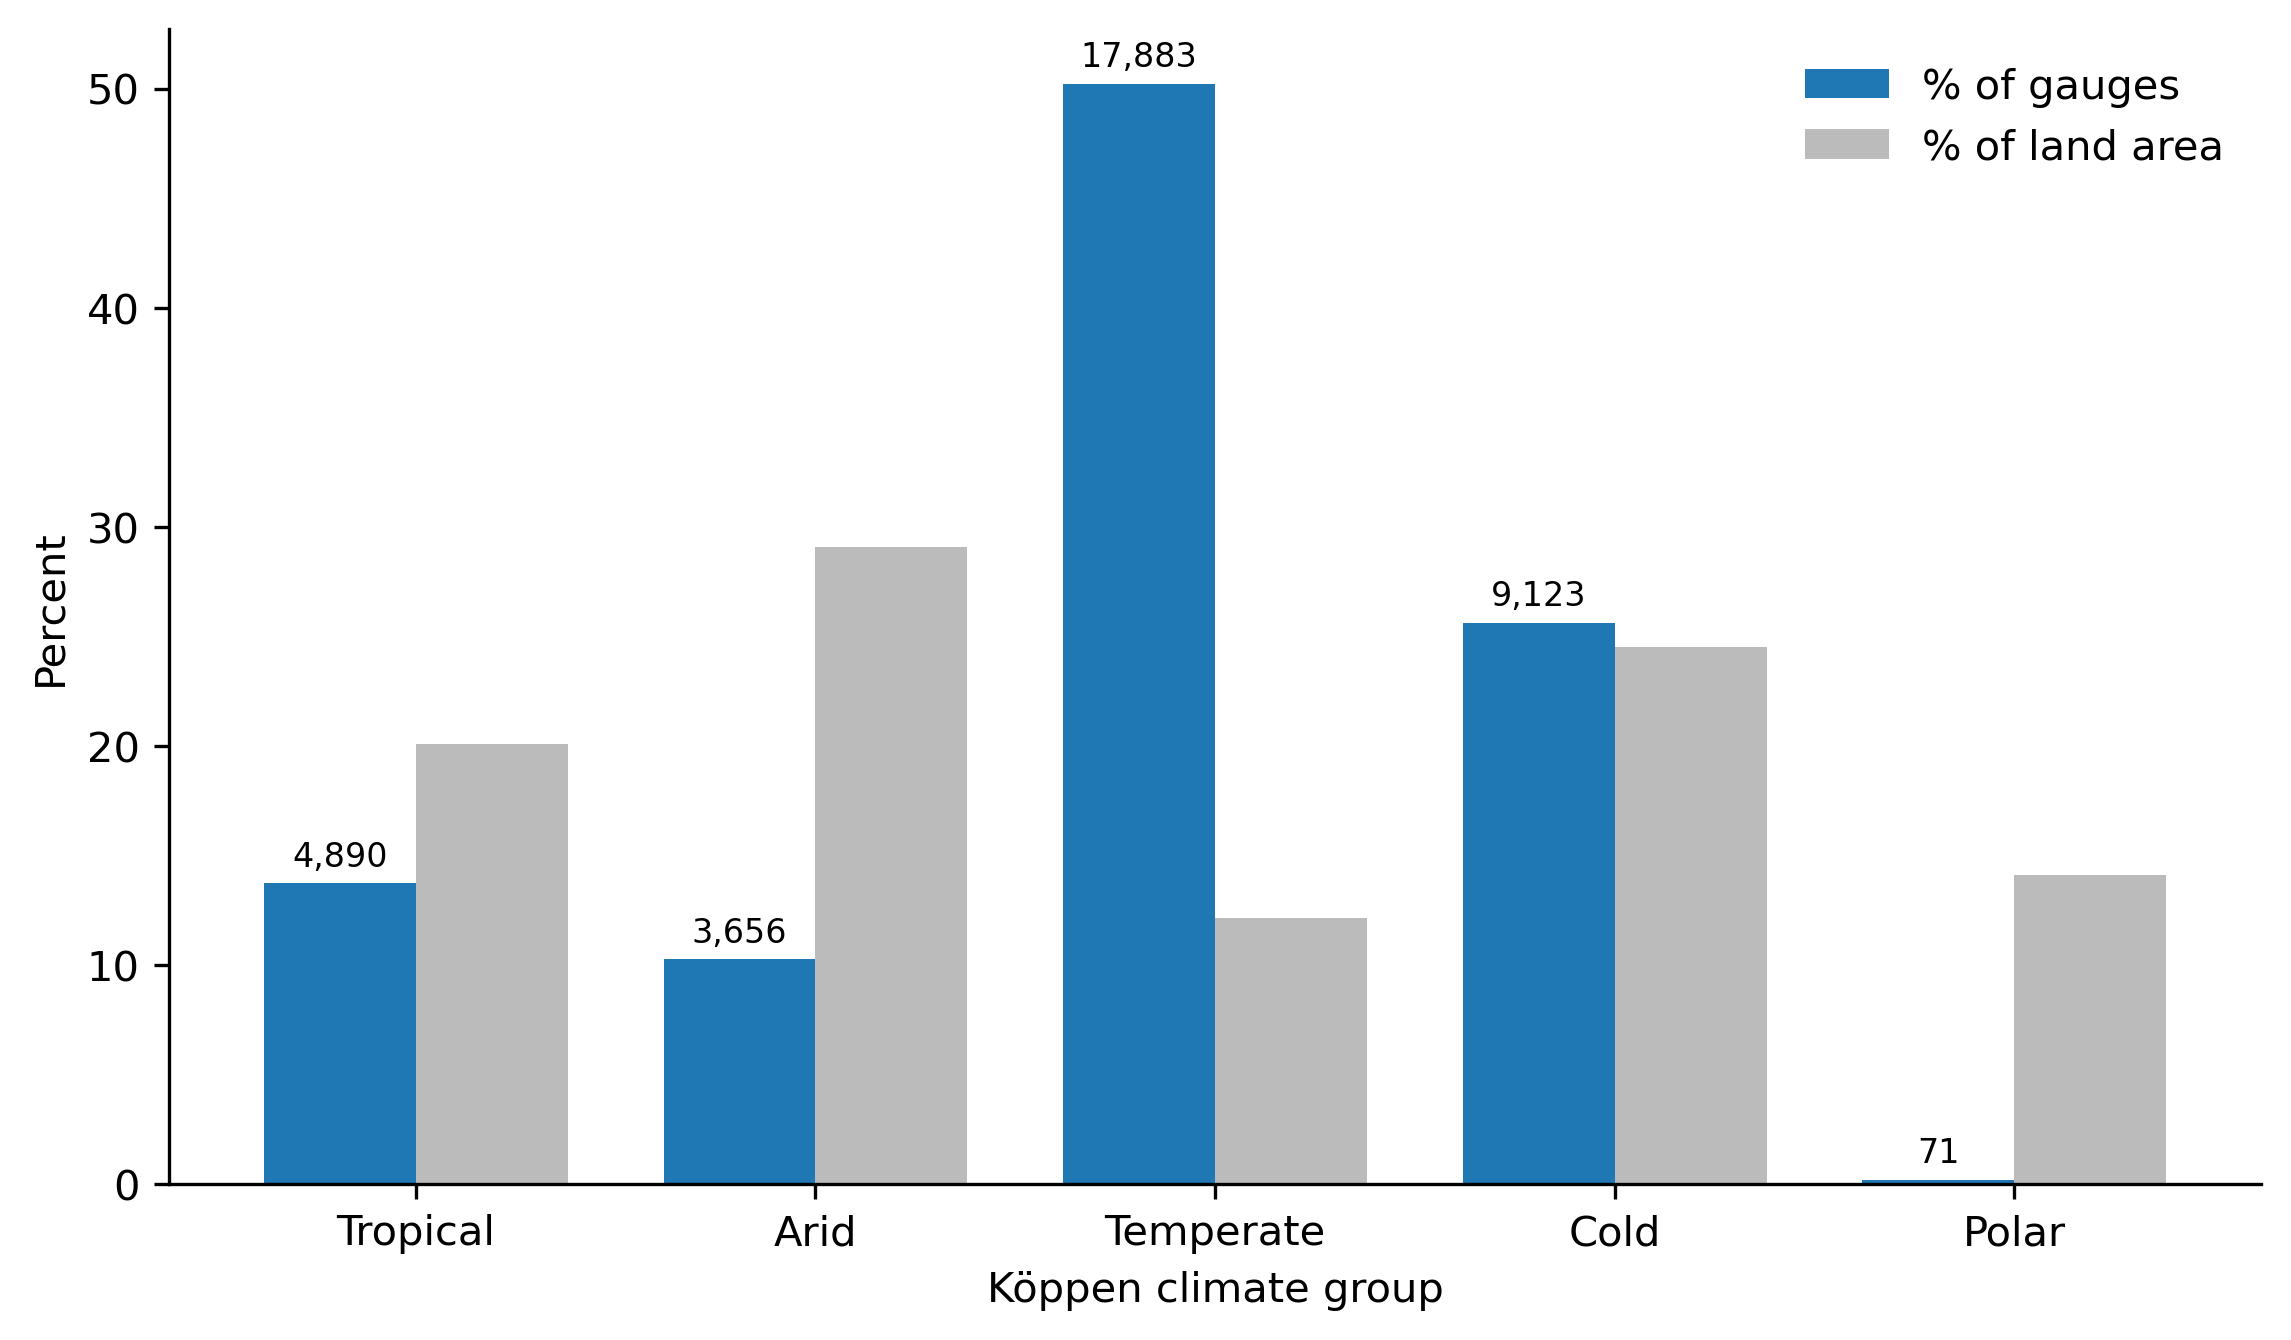
\includegraphics[width=\textwidth]{figures/fig04_koppen_climate.png}
\caption{Total number of gauges per Koppen climate category.}
\label{fig:koppen}
\end{figure}

The gauges in the dataset are matched with RFS streams. (\emph{Describe in more depth?}) All gauges that have been matched used this global hydrology to show what areas are covered by a gauges. And area is covered by a gauge if there is any gauge downstream of that river. The following map displays the results of this analysis.

% [Word comment] Something is wrong because I think we do have gauges in a
% couple spots that aren't showing
\begin{figure}[!htbp]
\centering
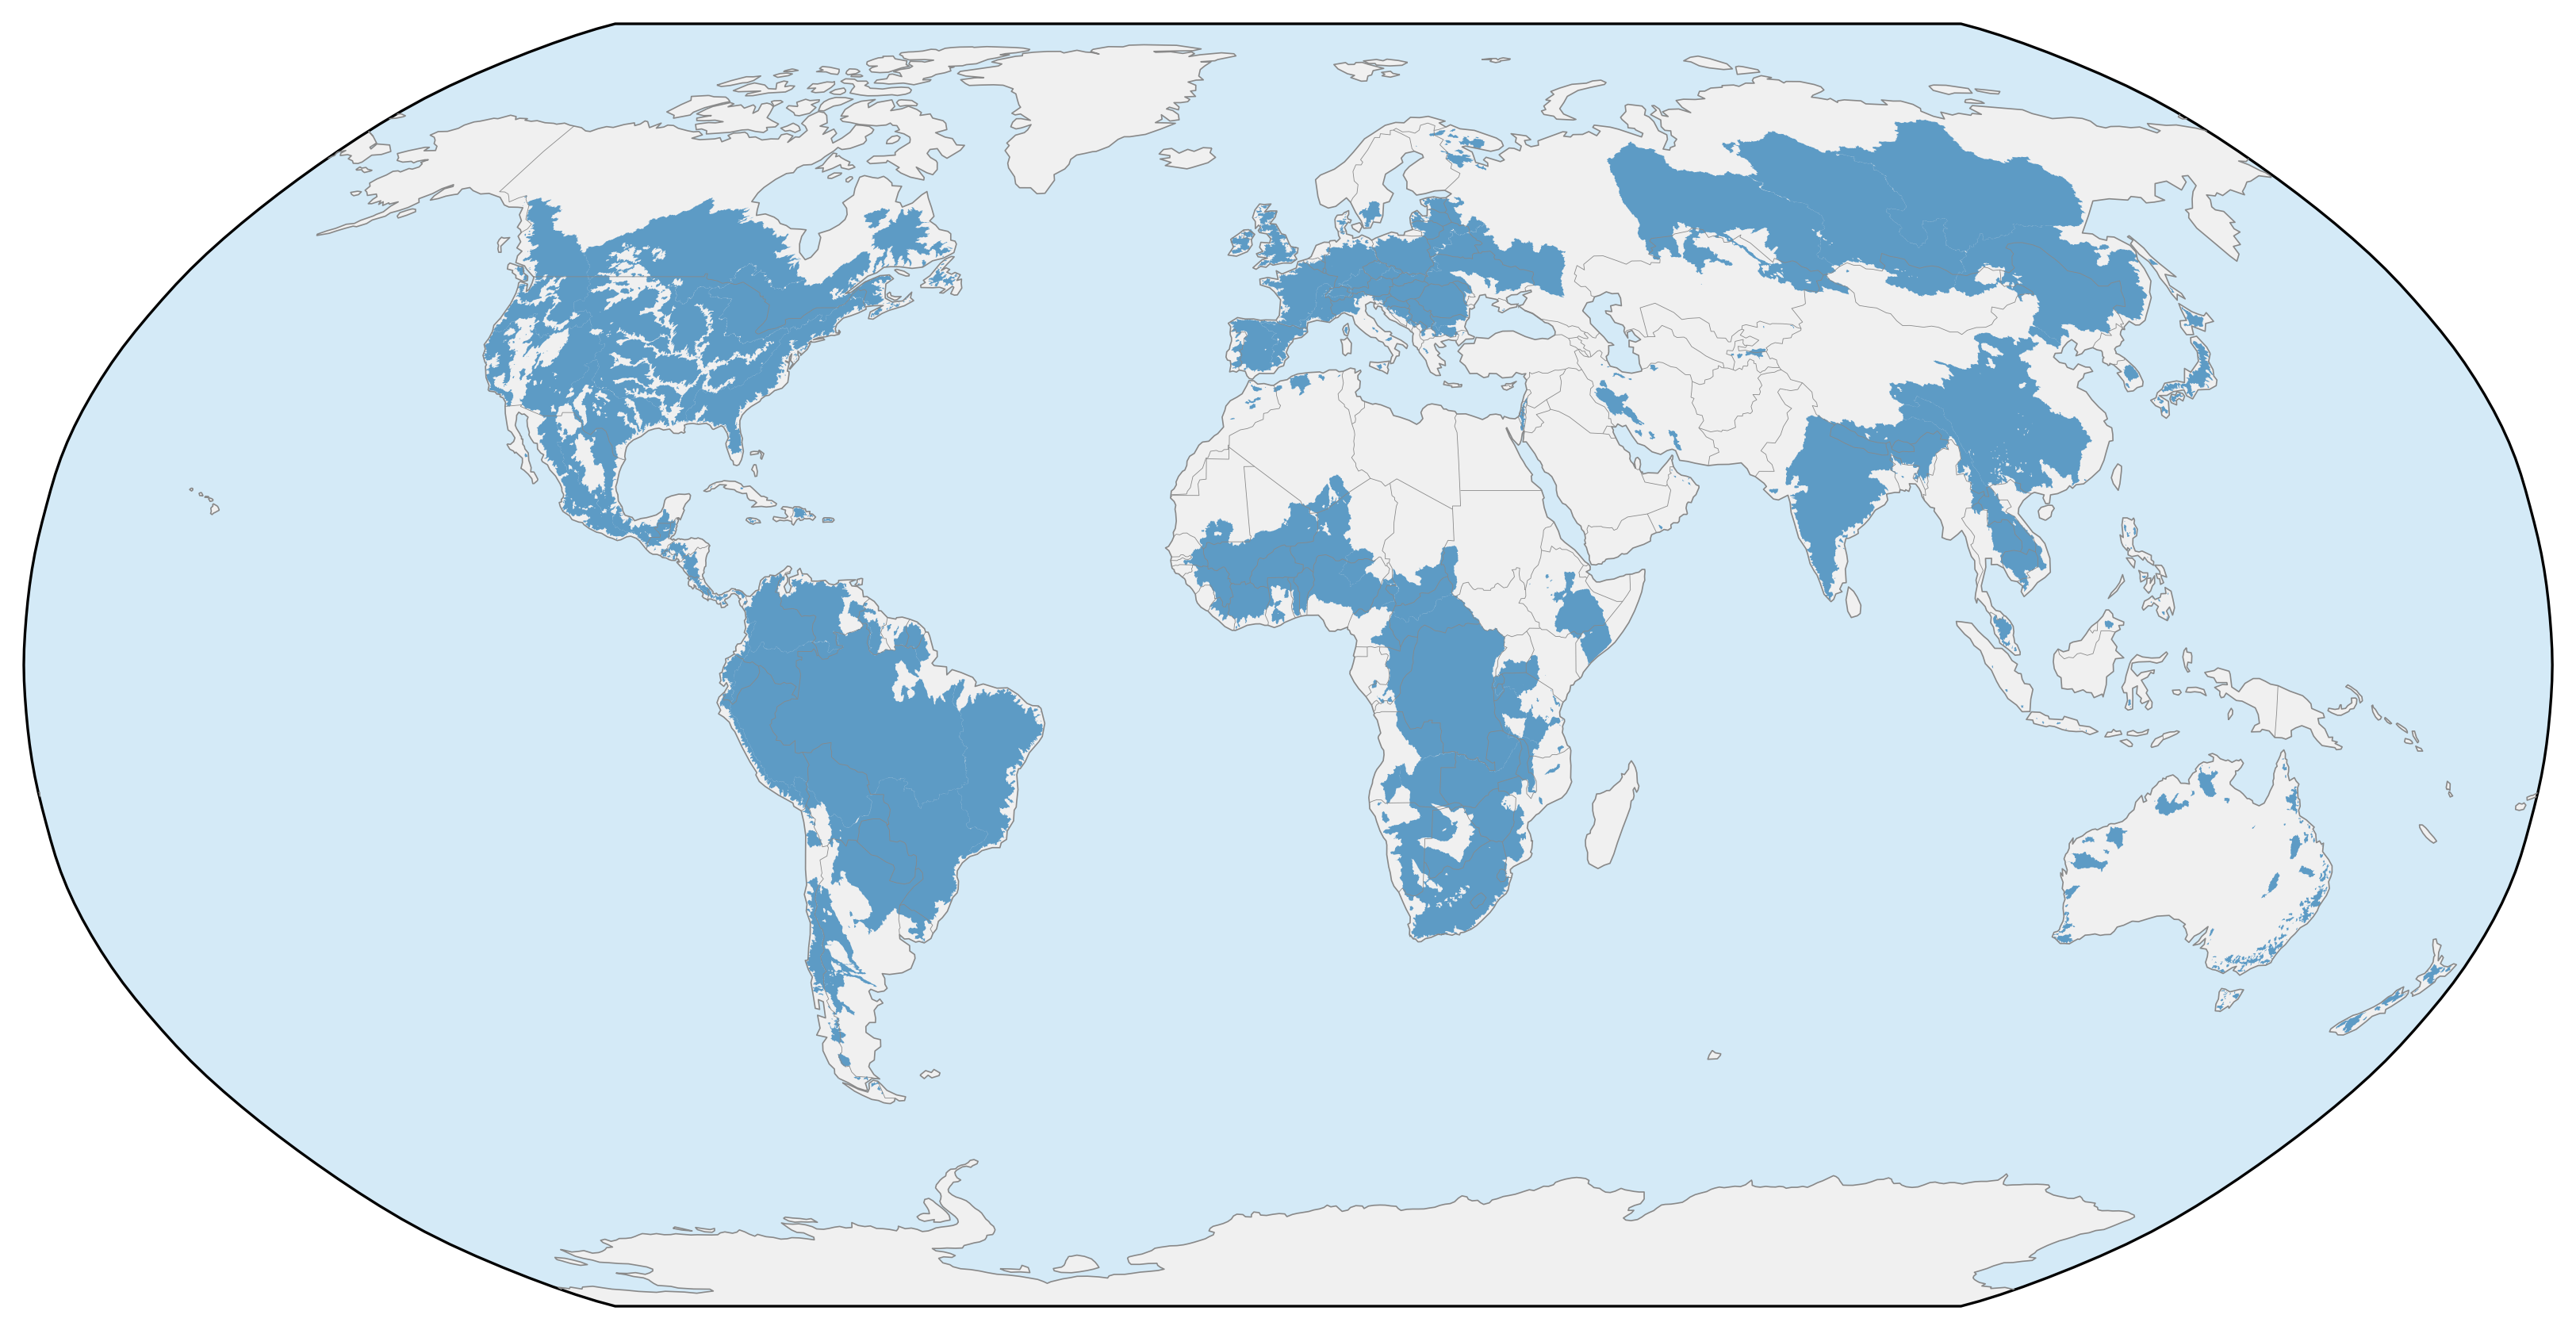
\includegraphics[width=\textwidth]{figures/fig05_gauge_coverage.png}
\caption{Watersheds with gauges.}
\label{fig:gauge-coverage}
\end{figure}

\begin{figure}[!htbp]
\centering
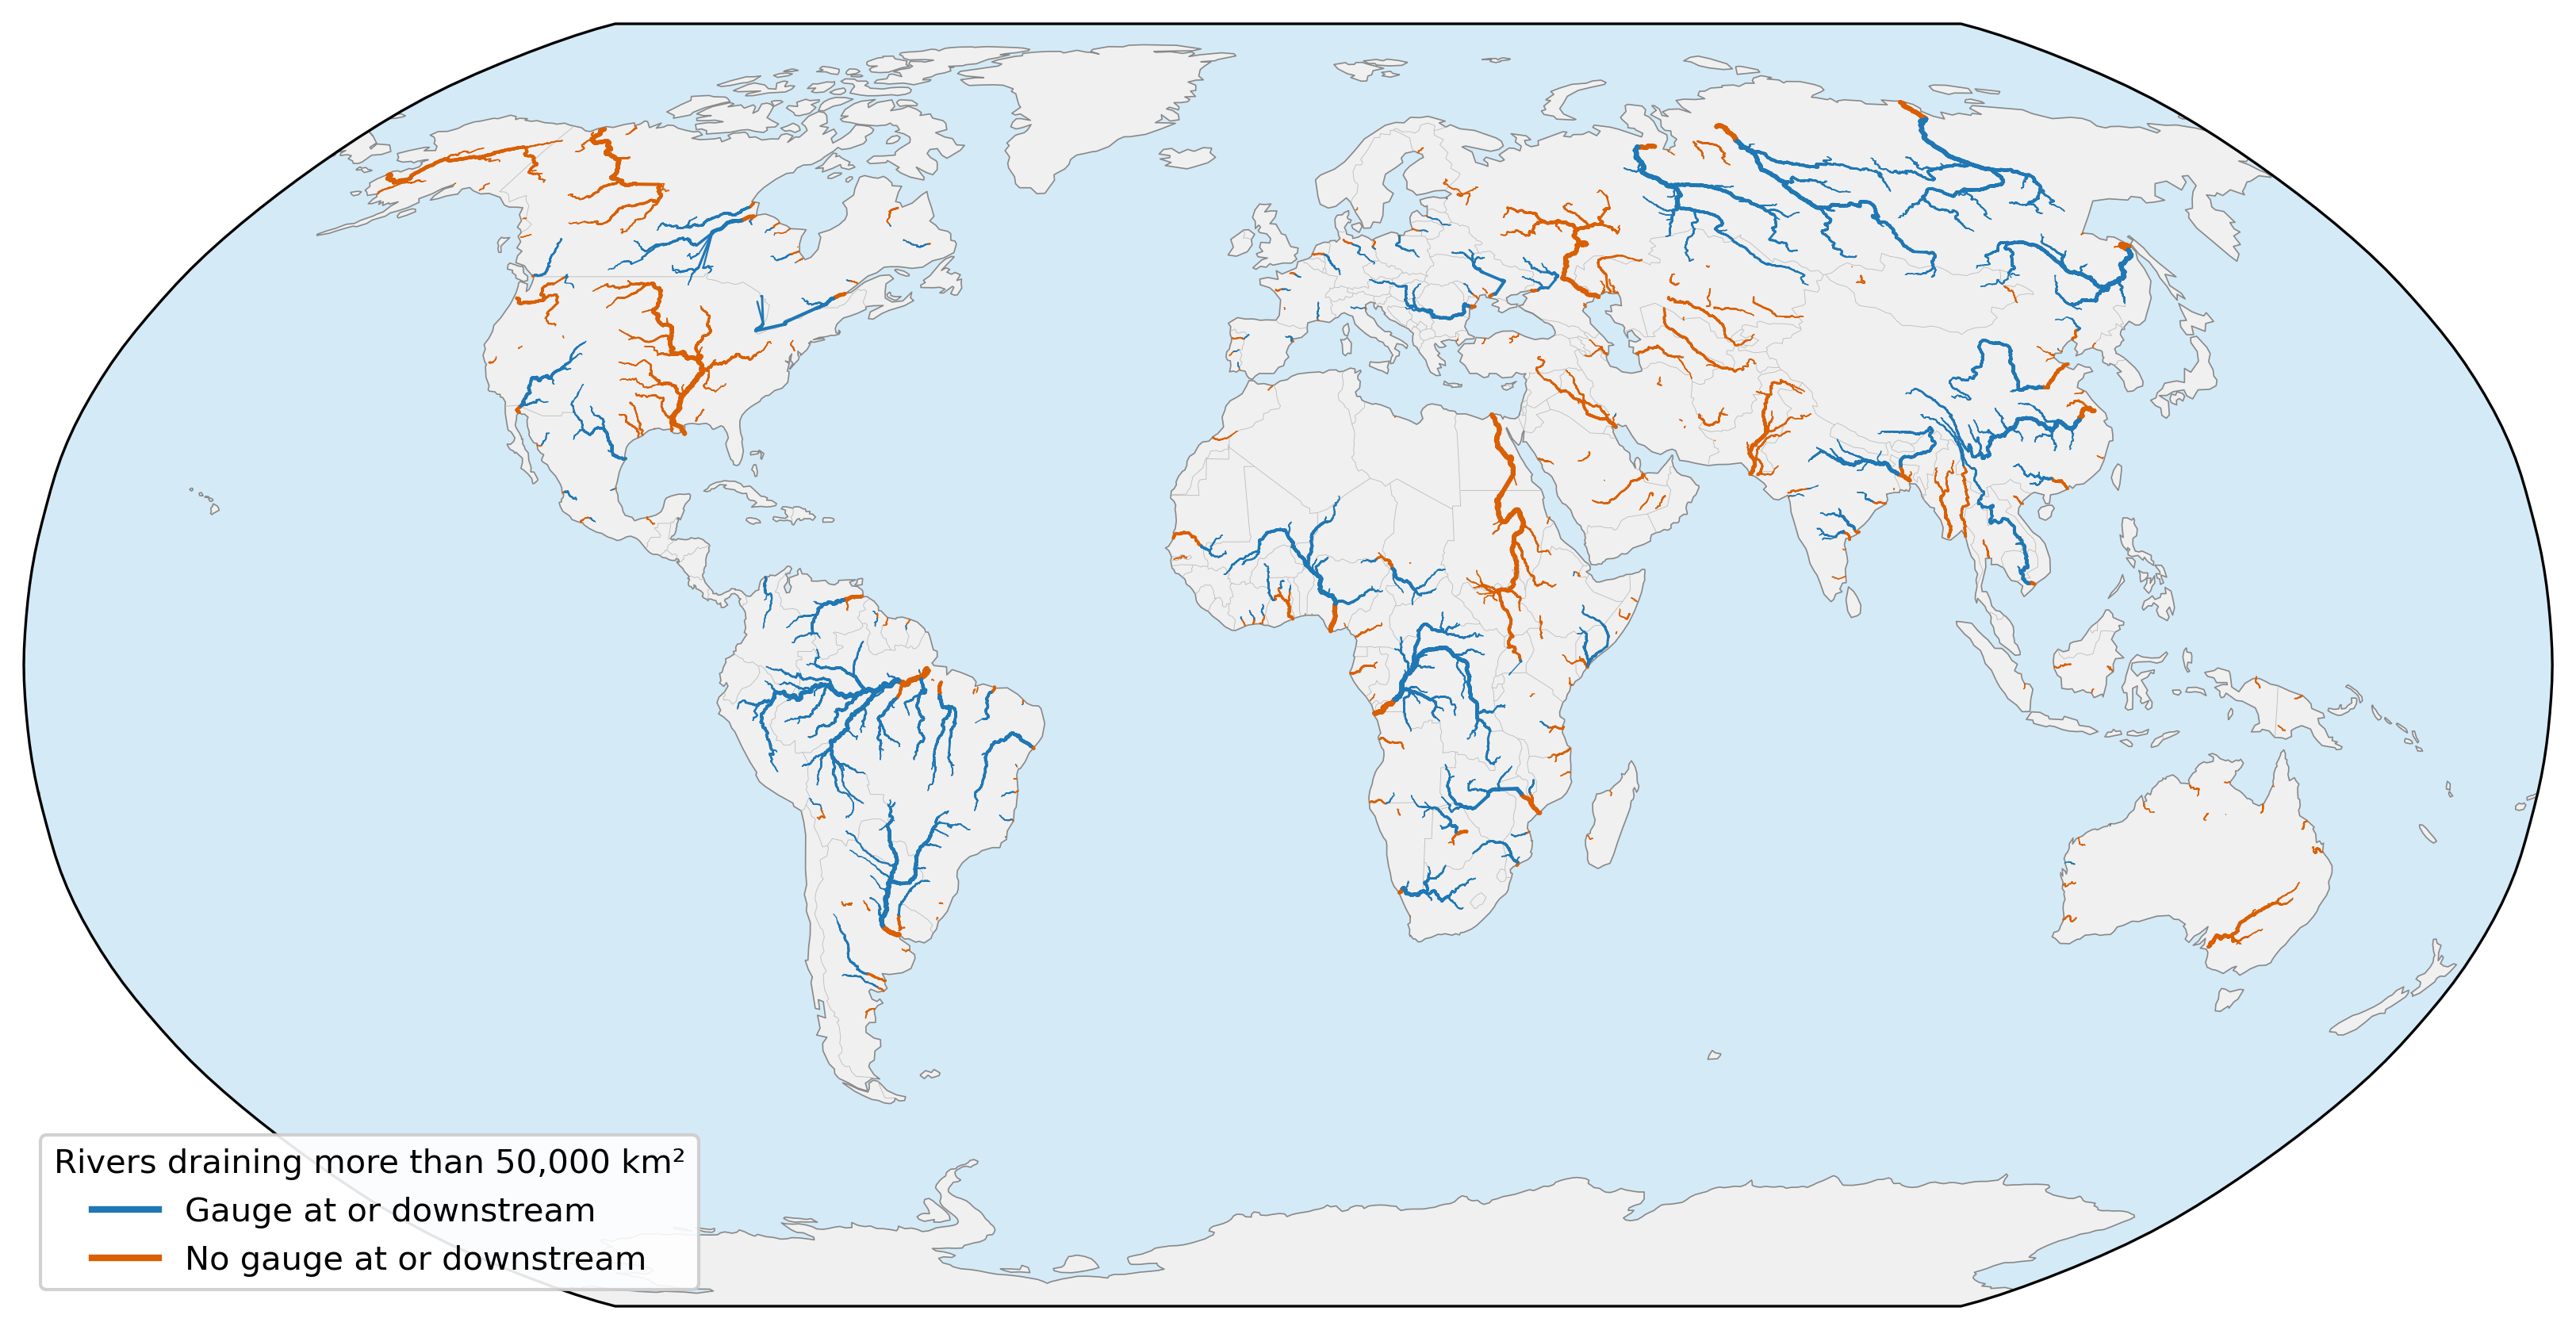
\includegraphics[width=\textwidth]{figures/fig06_large_river_coverage.png}
\caption{Rivers draining more than 50,000~km\textsuperscript{2}, coloured by whether a gauge is at or downstream of them (the same rule as Figure~\ref{fig:gauge-coverage}). Line width grows with upstream area.}
\label{fig:large-river-coverage}
\end{figure}

These figures show that there are a couple major rivers that either have no gauges in the watershed or only have it on upstream segments. The Nile, Volga, Tigis-Euphrates, and Indus are all rivers that do not have gauges on their main tributaries. 

\emph{Slice and dice fifty ways.}

\emph{Watersheds that have rivers}

\emph{How many gages do we know about that are not in our database (e.g., China, Russia, Nile, the stans, Indus, Tigris, Euphrates, Paraná}

\emph{ALASKA?}

\emph{Places where we have no GeoGlows stream reach for a gage. (QUESTION: Who does have a model for that location? (e.g., does GloFAS or Flood Hub include that number of gages?)}

\emph{Continent -- world bank regions? Hard to find specific continent shapefiles}

\subsection{Temporal Analysis -- When are the data?}
% [Word comment] The plots are based on Yubin's old data table. Concerned about
% its quality though!
% [Word comment] master_catalog.xls does not have temporal attributes like
% Start date and End date!

\draftnote{Temporal resolution -- how frequently are most of the measurements}

% [Word comment] 9150 gauges out of 37528 have missing start_date and/or
% end_date which led to their exclusion in temporal analysis.
This section presents temporal analyses of the globally distributed gauge dataset compiled in this research. As shown in Table~\ref{tab:temporal}, temporal coverage varies substantially across regions, reflecting historical differences in hydrological monitoring investment and institutional capacity. Europe and North America hold the deepest historical records, with gauges dating back to 1806 and 1862, respectively, and together account for over 95\% of gauging stations predating 1930. Africa, South America, and Australia each contribute modest pre-1930 representation in tens of stations, while Asia, South Asia, and Central America contribute fewer than 10 gauges before that mark. The Middle East stands apart as the only region with no gauge records before 1983. Because pre-1930 coverage is concentrated almost entirely in Europe and North America, temporal analysis in this study begins in 1930, after which enough regions have established monitoring records to support meaningful cross-regional comparison. Further, record availability extends through the early-to-mid 2020s across most regions, with North America and Central America offering the most current data through 2025, and Asia and the Middle East trailing with records last updated through 2021.

Sub-daily measurement availability follows a similarly uneven pattern: Australia and South America lead with 63.2\% and 52.1\% of their gauges providing sub-daily data, while Africa, Asia, the Middle East, South Asia, and Central America report none. These disparities suggest that data-sparse regions not only lack spatial gauge density but also suffer from shallower temporal records and coarser measurement resolution, compounding the challenge of using observational data for global hydrological model calibration and validation in those areas.

\begin{table}[!htbp]
\centering
\caption{Temporal coverage of gauge records by region.}
\label{tab:temporal}
\small
\begin{tabular}{@{}lC{0.15\textwidth}C{0.15\textwidth}C{0.15\textwidth}C{0.15\textwidth}@{}}
\toprule
\textbf{Region} & \textbf{Earliest gauge date} & \textbf{Latest gauge date} & \textbf{Number of Gauges before 1930} & \textbf{\% Gauges with subdaily data} \\
\midrule
Africa & 1903 & 2024 & 41 & 0 \\
Asia & 1902 & 2021 & 7 & 0 \\
Australia & 1905 & 2022 & 18 & 63.2 \\
Central America & 1936 & 2025 & 0 & 0.2 \\
Europe & 1806 & 2024 & 707 & 26.3 \\
Middle East & 1983 & 2021 & 0 & 0 \\
North America & 1862 & 2025 & 1468 & 24 \\
South America & 1901 & 2022 & 44 & 52.1 \\
South Asia & 1913 & 2024 & 2 & 0 \\
\bottomrule
\end{tabular}
\end{table}

Figure~\ref{fig:active-gauges} shows the number of active gauges per region from 1930 to the latest gauge available year. North America and Europe dominate the global gauge network throughout this period, with North America peaking at approximately 9,000 active gauges around 1990 and Europe reaching roughly 5,500 by the mid-2010s. The rise in the number of gauges globally around 1980 can be attributed to the WMO and UNESCO initiatives to expand global hydrological monitoring following the International Hydrological Decade (1965--1974) \citep{more1980}. Studies on dams reveal that the construction of dams peaked globally between the 1960s and 1980s \citep{perera2021}, which could have caused a proportional increase in gauging stations.

% [Word comment] (on "Both regions exhibit a marked decline") This decline is
% really huge and there must be some reasons. / Look for those.
% [Word comment] (on "1980,") Find the possible reason for the sharp rise in
% number of gauges in different regions.
Both regions exhibit a marked decline in active gauges after approximately 2015, suggesting either network contraction or reporting lags in recently compiled data. South America shows a notable expansion beginning around 1980, rising from near zero to approximately 1,500 active gauges, where it remains relatively stable through 2020. All other regions --- Africa, Asia, Australia, Central America, the Middle East, and South Asia --- maintain consistently low gauge counts throughout the entire period, remaining nearly indistinguishable from zero on this scale. The major decline in freshwater monitoring networks stems primarily from insufficient funding and shifting government priorities \citep{ruhi2018}.

This persistent underrepresentation underscores the severe temporal and spatial data gaps that characterize the global gauge network outside of North America and Europe, with direct implications for the reliability of global hydrological models in those regions.

\begin{figure}[!htbp]
\centering
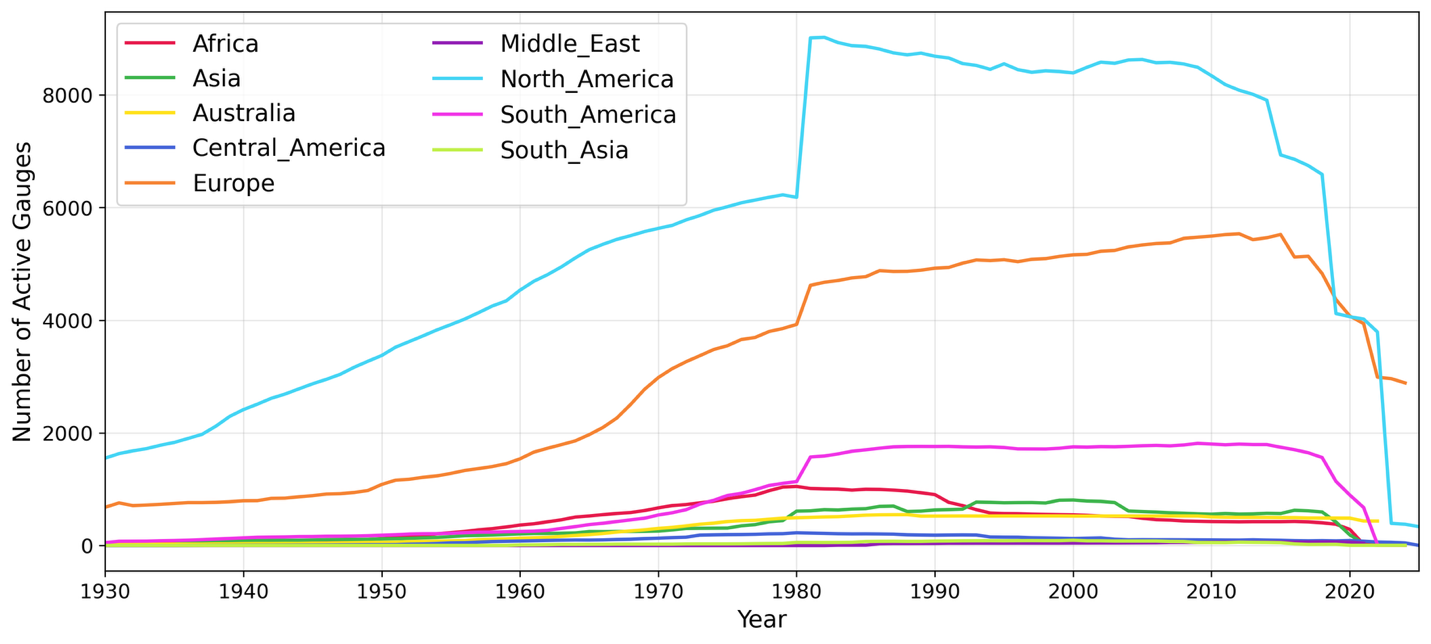
\includegraphics[width=\textwidth]{figures/fig07_active_gauges_by_region.png}
\caption{Number of active gauges per region from 1930 to the latest year with available data.}
\label{fig:active-gauges}
\end{figure}

The decadal heatmap of active gauges (Figure~\ref{fig:decadal-heatmap}) by region reveals distinct trajectories in global monitoring capacity over the past nine decades. North America reached peak coverage in the 1980s with 8,862 active gauges, followed by a gradual decline to 6,935 in the 2010s. Europe shows the most consistent growth trajectory, expanding from 747 gauges in the 1930s to 5,522 in the 2010s without interruption. Africa, by contrast, peaked in the 1980s at 999 gauges and has since declined to 424 in the 2010s, representing a more than 50\% reduction in active monitoring capacity over four decades. South America grew steadily through the 1980s and has remained relatively stable since, while Central America, Australia, and Asia maintain a modest but measurable presence. The Middle East and South Asia remain severely underrepresented throughout the entire period, with the Middle East recording zero active gauges before the 1980s and South Asia never exceeding 85 gauges in any decade. Taken together, these patterns reveal that global gauge network expansion was largely a mid-twentieth century phenomenon concentrated in the Global North, with several regions now experiencing declining coverage rather than growth.

\begin{figure}[!htbp]
\centering
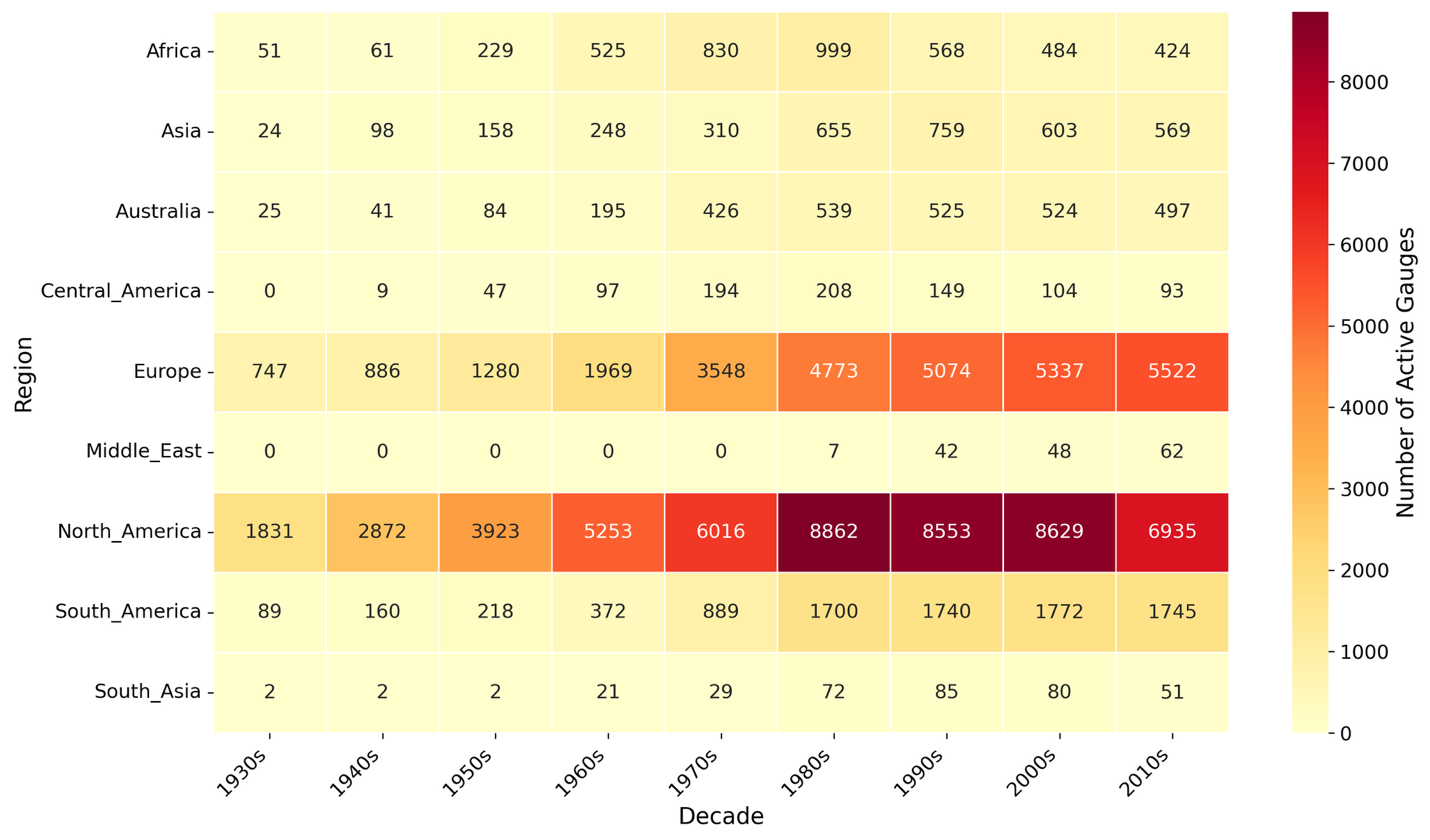
\includegraphics[width=\textwidth]{figures/fig08_decadal_heatmap.png}
\caption{Decadal heatmap of active gauges by region.}
\label{fig:decadal-heatmap}
\end{figure}

Figure~\ref{fig:starts-ends} illustrates the annual number of gauges beginning and ending operation between 1930 and 2024. We assumed the gauges to be active at present if the gauges were active on the date of last measurement. From 1930 through the late 1970s, new gauge installations consistently outpaced closures, reflecting the global expansion of hydrological monitoring networks during the mid-twentieth century. A pronounced spike of approximately 4,100 gauge starts occurs around 1980, the origins of which warrant further investigation but may reflect a coordinated international monitoring initiative or a major data contribution from a single national agency during that period. Beginning in the mid-1980s, gauge endings become increasingly frequent, and the balance between new starts and closures shifts toward net loss. This decline accelerates markedly in the late 2010s, with a peak of nearly 3,000 gauge endings recorded around 2018--2019. While some portion of this recent decline may reflect genuine network contraction, it is likely also attributable to reporting lags in recently compiled data, where records for active gauges have not yet been updated through the present. Nonetheless, the overall trajectory is clear: global gauge network growth stalled and in many regions reversed after the mid-1980s, with implications that are particularly severe for data-sparse regions that never achieved adequate coverage to begin with.

\begin{figure}[!htbp]
\centering
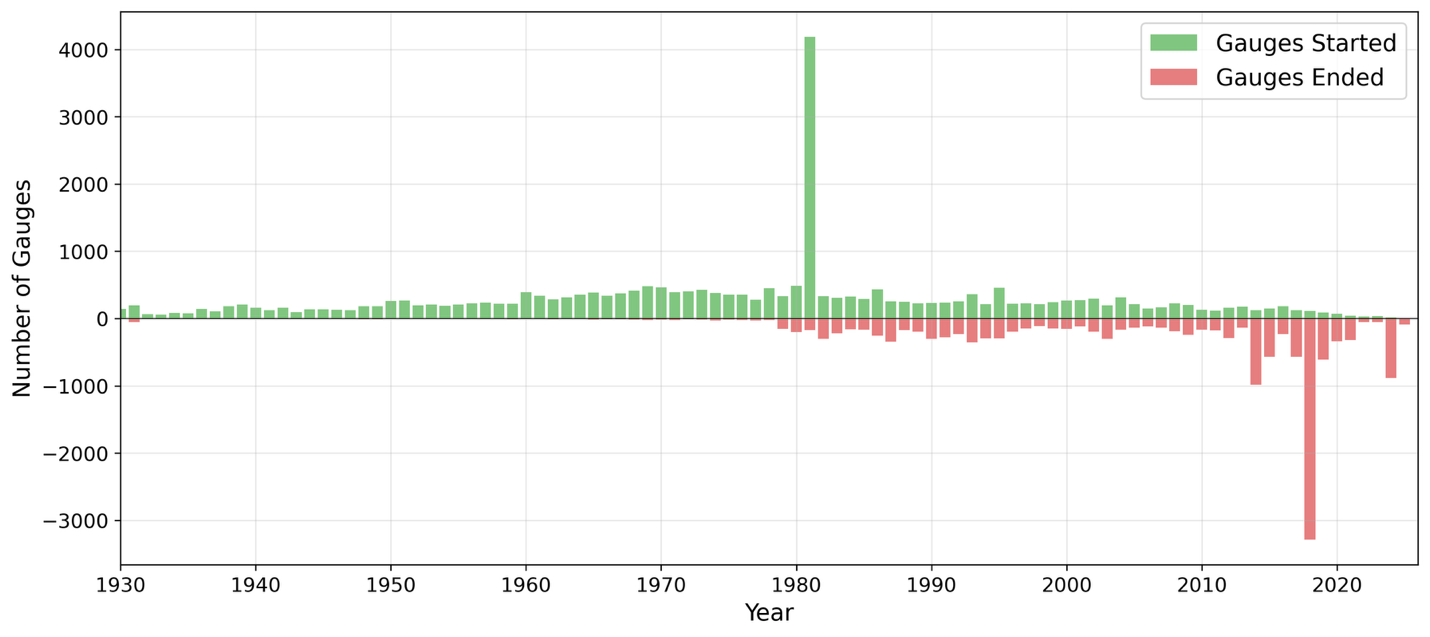
\includegraphics[width=\textwidth]{figures/fig09_gauge_starts_ends.png}
\caption{Annual number of gauges beginning and ending operation, 1930--2024.}
\label{fig:starts-ends}
\end{figure}

Figure~\ref{fig:record-duration} shows the distribution of gauge record durations by region, expressed as a percentage of stations within each duration category. Europe and North America demonstrate the most favorable duration profiles, with large proportions of stations operating for 30 years or more --- the threshold commonly recommended by the World Meteorological Organization for reliable hydrological analysis. North America notably contains the highest share of records exceeding 100 years, reflecting its long institutional history of systematic streamflow monitoring. In contrast, the Middle East is heavily weighted toward short-duration records of fewer than 10 years, consistent with its late network establishment in the 1980s. Asia exhibits a disproportionately large share of very short records of under five years, compounding the data quality concerns identified in the missing data analysis. Africa, despite having gauges dating to the early twentieth century, shows a substantial proportion of short-duration records, suggesting significant discontinuity and gauge turnover within its network over time. Australia and South America present more balanced duration profiles, with meaningful representation in the 20--50 year range. Taken together, these distributions indicate that outside of Europe and North America, a large fraction of the global gauge network does not meet minimum duration thresholds for robust hydrological modeling, further constraining the utility of available data in regions where observational coverage is already limited.

\draftnote{Some relevant research papers for this section}

\citep{lanfear1999} talks about how USGS gauges are changing with time

\citep{ruhi2018} talks about decline in global gauge networks

\begin{figure}[!htbp]
\centering
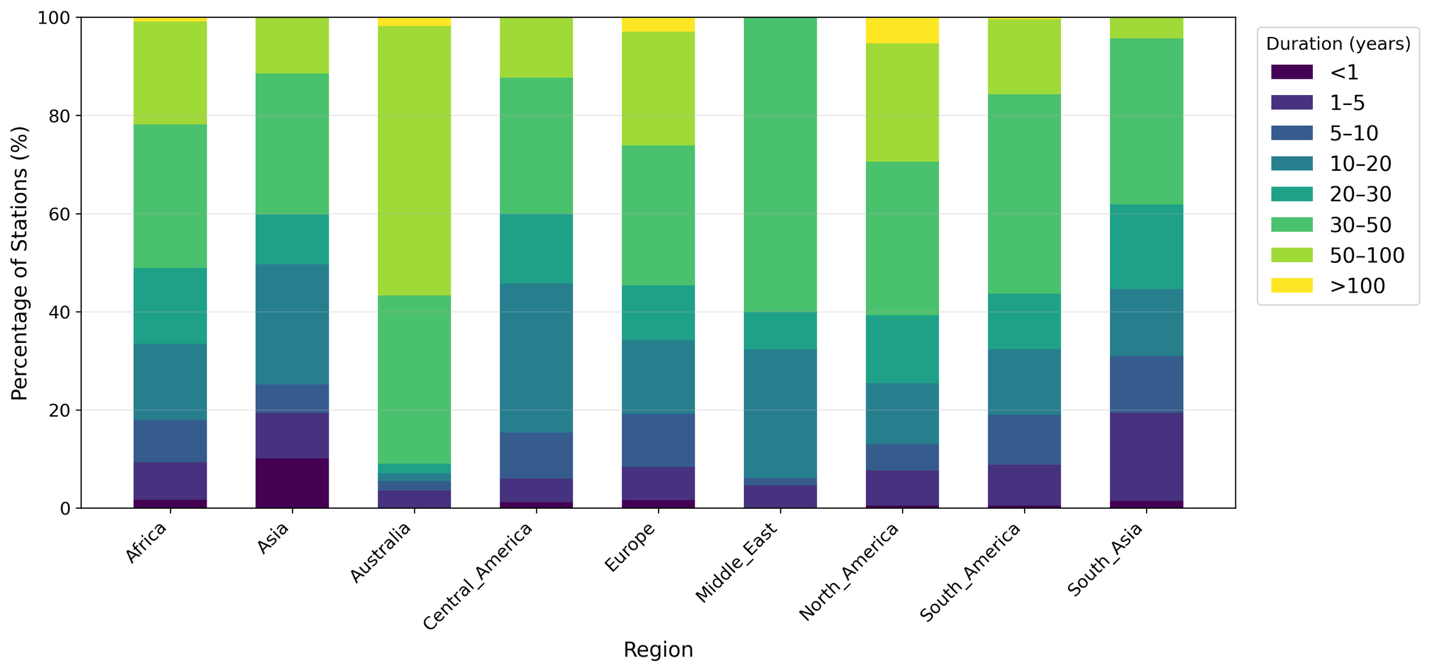
\includegraphics[width=\textwidth]{figures/fig10_record_duration.png}
\caption{Distribution of gauge record durations by region, expressed as a percentage of stations within each duration category.}
\label{fig:record-duration}
\end{figure}

Figure~\ref{fig:missing-data} presents the distribution of missing data percentages across gauge records by region, offering insight into data quality independent of network size. Australia and the Middle East demonstrate the highest record completeness, with median missing data rates near zero, suggesting that where gauges exist in these regions, their records are generally well maintained. North America and Europe similarly show low median missingness, though both exhibit long upper whiskers extending to 100\%, indicating that a subset of gauges within these otherwise data-rich regions have severely incomplete records. Asia shows the poorest typical data quality, with a median missing data rate of approximately 38\% and a wide interquartile range, meaning that even where gauge records exist, substantial portions are often unavailable. Central America and Africa show intermediate but concerning levels of missingness, with medians near 30\% and 15--20\% respectively and numerous high-value outliers. Notably, the Middle East and South Asia --- regions with the fewest gauges overall --- do not exhibit the worst data quality, suggesting that network scarcity and record incompleteness are distinct but compounding challenges. Together, these findings indicate that the effective data available for hydrological modeling is considerably less than raw gauge counts alone would suggest.

% [Word comment] This plot is based on Yubin's table.
% [Word comment] What is the time step of the higher temporal resolution data
% available?
% [Word comment] Asia and South Asia separate??
\begin{figure}[!htbp]
\centering
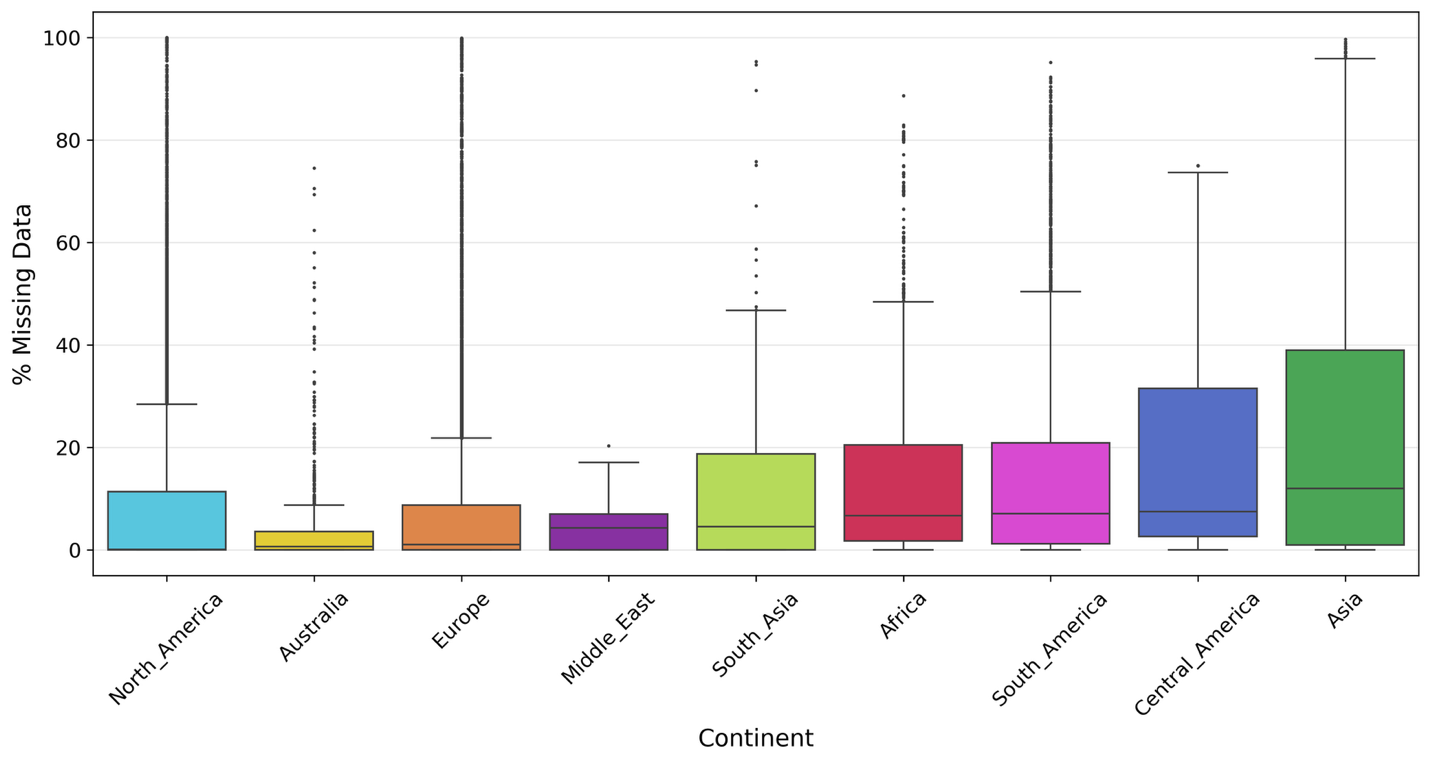
\includegraphics[width=\textwidth]{figures/fig11_missing_data.png}
\caption{Distribution of missing data percentages across gauge records by region.}
\label{fig:missing-data}
\end{figure}

\draftnote{Some relevant research papers for this section}

\citep{lanfear1999} talks about how USGS gauges are changing with time

\citep{ruhi2018} talks about decline in global gauge networks

% ===========================================================================
